\chapter{线性规划与规约 (Linear programming and reductions)}

在许多计算任务中，我们的目标是在满足一系列给定的硬性约束条件下，寻找能够最大化收益或最小化成本的最优资源分配方案。如果这些约束条件以及目标函数都可以表示为变量的线性等式或线性不等式，那么该问题就属于\textbf{线性规划 (Linear Programming，简称 LP)}。线性规划是应用数学和算法设计中最强大的普适性工具之一，它不仅自身拥有多项式时间解法，更是解决网络流、二分匹配、零和博弈等众多核心问题的“万能转换器”。

\section{线性规划引论 (An introduction to linear programming)}

考虑一个典型的生产优化示例：某工厂生产两种产品 $x_1$ 和 $x_2$。每生产一单位 $x_1$ 获利 1 美元，每生产一单位 $x_2$ 获利 6 美元。生产过程受到三项资源限制：
\begin{align*}
x_1 &\le 200 & (\text{原料 A 供应限制}) \\
x_2 &\le 300 & (\text{原料 B 供应限制}) \\
x_1 + x_2 &\le 400 & (\text{总工时限制}) \\
x_1, x_2 &\ge 0 & (\text{产量非负约束})
\end{align*}
工厂的目标是最大化总利润：$\max (x_1 + 6x_2)$。

\begin{figure}[htbp]
\centering
\begin{tikzpicture}[scale=0.85, >=latex]
    \draw[->] (0,0) -- (5,0) node[right] {$x_1$};
    \draw[->] (0,0) -- (0,5) node[above] {$x_2$};
    % 约束边界
    \draw[thick, blue] (2,0) -- (2,4) node[above] {$x_1 = 200$};
    \draw[thick, red] (0,3) -- (4,3) node[right] {$x_2 = 300$};
    \draw[thick, green!60!black] (0,4) -- (4,0) node[right] {$x_1 + x_2 = 400$};
    
    % 可行域填充
    \fill[gray!20, opacity=0.7] (0,0) -- (2,0) -- (2,2) -- (1,3) -- (0,3) -- cycle;
    \draw[very thick] (0,0) -- (2,0) -- (2,2) -- (1,3) -- (0,3) -- cycle;
    
    % 顶点标记
    \node[circle,fill=black,inner sep=1.2pt,label=below left:{(0,0)}] at (0,0) {};
    \node[circle,fill=black,inner sep=1.2pt,label=below:{(200,0)}] at (2,0) {};
    \node[circle,fill=black,inner sep=1.2pt,label=right:{(200,200)}] at (2,2) {};
    \node[circle,fill=red,inner sep=2pt,label=above right:{\textbf{最优解 (100,300)}}] at (1,3) {};
    \node[circle,fill=black,inner sep=1.2pt,label=left:{(0,300)}] at (0,3) {};
    
    % 目标函数等值线
    \draw[dashed, thick, orange] (-0.5, 3.25) -- (2.5, 2.75) node[right] {$x_1 + 6x_2 = 1900$};
\end{tikzpicture}
\caption{二维线性规划的可行域（凸多边形）与最优极点}
\label{fig:lp_2d}
\end{figure}

在几何上，每个线性不等式在空间中定义了一个半空间，所有不等式约束的交集构成了一个凸多面体（在二维空间中为凸多边形），称为\textbf{可行域 (feasible region)}。目标函数的等值线是一族平行的超平面。沿着目标函数增加的方向平移该超平面，最后一个与可行域保持接触的点必然位于该多面体的\textbf{顶点（极点，vertex）}上！

\begin{property}
若线性规划存在有限的最优解，则必存在一个最优解在可行域多面体的某个顶点处取得。
\end{property}

\begin{sidebarbox}{矩阵与向量记号 (Matrix-vector notation)}
一般的线性规划标准型可以极其紧凑地表示为向量和矩阵乘积形式：
\begin{align*}
\max \quad & \bm{c}^T \bm{x} \\
\text{s.t.} \quad & \bm{A}\bm{x} \le \bm{b} \\
& \bm{x} \ge \bm{0}
\end{align*}
其中 $\bm{x} \in \mathbb{R}^n$ 是待求解的决策变量向量，$\bm{c} \in \mathbb{R}^n$ 为目标函数系数向量，$\bm{A} \in \mathbb{R}^{m \times n}$ 为约束系数矩阵，$\bm{b} \in \mathbb{R}^m$ 为资源常数项向量。
\end{sidebarbox}

\section{网络流 (Flows in networks)}

在计算机网络或供水系统中，我们希望从指定的源点 $s$ 向汇点 $t$ 输送尽可能多的流量。有向图中的每条边 $e = (u, v)$ 具有容量上限 $c_e > 0$。

\begin{tcolorbox}[colback=white,colframe=gray!50!black]
\textbf{最大流问题 (Maximum Flow)} \\
\textbf{变量：} 每条边 $e \in E$ 上的流量 $f_e$。 \\
\textbf{目标：} $\max \sum_{(s, u) \in E} f_{su}$（最大化从源点流出的净流量） \\
\textbf{约束条件：}
\begin{enumerate}
    \item \textbf{容量约束 (Capacity constraints)}：对所有 $e \in E$，$0 \le f_e \le c_e$；
    \item \textbf{流量守恒 (Conservation of flow)}：对所有除 $s, t$ 之外的内部节点 $u \in V \setminus \{s, t\}$：
    \[
    \sum_{(v, u) \in E} f_{vu} = \sum_{(u, w) \in E} f_{uw}.
    \]
\end{enumerate}
\end{tcolorbox}

由于目标函数与约束条件全部是关于变量 $f_e$ 的线性的，最大流问题可以直接看作是一个特殊的线性规划问题！

\begin{figure}[htbp]
\centering
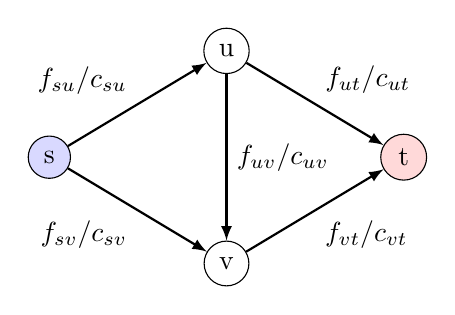
\begin{tikzpicture}[scale=0.9, auto, >=latex]
    \node[circle,draw,fill=blue!15] (s) at (0,1.5) {s};
    \node[circle,draw] (u) at (2.5,3) {u};
    \node[circle,draw] (v) at (2.5,0) {v};
    \node[circle,draw,fill=red!15] (t) at (5,1.5) {t};

    \draw[->,thick] (s) -- node[above left] {$f_{su}/c_{su}$} (u);
    \draw[->,thick] (s) -- node[below left] {$f_{sv}/c_{sv}$} (v);
    \draw[->,thick] (u) -- node[right] {$f_{uv}/c_{uv}$} (v);
    \draw[->,thick] (u) -- node[above right] {$f_{ut}/c_{ut}$} (t);
    \draw[->,thick] (v) -- node[below right] {$f_{vt}/c_{vt}$} (t);
\end{tikzpicture}
\caption{流网络示意图（每条边标注为“当前流量/容量上限”）}
\label{fig:flow_network}
\end{figure}

\subsection*{Ford-Fulkerson 增广路算法与最大流最小割定理}
对于当前流 $f$，我们构建\textbf{残量网络 (residual network)} $G_f$：每条前向剩余容量为 $c_e - f_e$ 的边允许继续正向增广，每条反向流量为 $f_e$ 的边允许退流回退。只要在 $G_f$ 中存在从 $s$ 到 $t$ 的有向路径（称为\textbf{增广路 (augmenting path)}），就可以沿着该路径增大总流量。

\begin{theorem}[\textbf{最大流最小割定理 (Max-Flow Min-Cut Theorem)}]
在任意网络流中，从源点 $s$ 到汇点 $t$ 的最大流值，严格等于分离 $s$ 和 $t$ 的所有割 $(S, T)$ 中的最小割容量 $\min_{(S, T)} \text{capacity}(S, T)$。
\end{theorem}

\section{二分图匹配 (Bipartite matching)}

给定一个二分图 $G = (V_1 \cup V_2, E)$，其中所有的边均连接 $V_1$ 中的节点与 $V_2$ 中的节点（例如求职者与工作岗位）。目标是找到一个边数最多的\textbf{匹配 (Matching)}，使得没有两条被选中的边共享公共端点。

\textbf{规约到最大流}：
\begin{enumerate}
    \item 引入超级源点 $s$，从 $s$ 向 $V_1$ 中的每个节点连一条容量为 1 的有向边；
    \item 将原二分图中的所有无向边转化为从 $V_1$ 指向 $V_2$ 的有向边，容量设为 1（或 $\infty$）；
    \item 引入超级汇点 $t$，从 $V_2$ 中的每个节点向 $t$ 连一条容量为 1 的有向边。
\end{enumerate}
在构造的网络上求解最大流，由于网络容量全为整数，流的\textbf{整数值性质 (Integrality property)} 保证了存在全整数解（流量非 0 即 1），从而求得的最大流值恰好等于最大二分匹配的大小！

\section{对偶性 (Duality)}

考虑一个求最大值的线性规划（称为\textbf{原问题 Primal}）：
\begin{align*}
\max \quad & 2x_1 + 3x_2 \\
\text{s.t.} \quad & x_1 + x_2 \le 4 \quad (\text{乘乘子 } y_1 \ge 0) \\
& x_1 + 3x_2 \le 9 \quad (\text{乘乘子 } y_2 \ge 0) \\
& x_1, x_2 \ge 0
\end{align*}
如果我们想证明目标函数的值绝不可能超过某个常数（寻找上界），可以将不等式进行线性组合：将第 1 个不等式乘以 $y_1$，第 2 个不等式乘以 $y_2$，两式相加得：
\[
(y_1 + y_2)x_1 + (y_1 + 3y_2)x_2 \le 4y_1 + 9y_2.
\]
只要乘子满足 $y_1 + y_2 \ge 2$ 且 $y_1 + 3y_2 \ge 3$，由于 $x_1, x_2 \ge 0$，就有：
\[
2x_1 + 3x_2 \le (y_1 + y_2)x_1 + (y_1 + 3y_2)x_2 \le 4y_1 + 9y_2.
\]
为了寻找最紧致的上界，我们希望最小化 $4y_1 + 9y_2$。这就导出了原问题的\textbf{对偶问题 (Dual LP)}：
\begin{align*}
\min \quad & 4y_1 + 9y_2 \\
\text{s.t.} \quad & y_1 + y_2 \ge 2 \\
& y_1 + 3y_2 \ge 3 \\
& y_1, y_2 \ge 0
\end{align*}

\begin{theorem}[\textbf{强对偶定理 (Strong Duality Theorem)}]
若原线性规划问题有最优解，则其对偶问题也必有最优解，且两者的最优目标函数值严格相等！
\[
\max \bm{c}^T \bm{x} = \min \bm{b}^T \bm{y}.
\]
\end{theorem}
最大流最小割定理正是强对偶定理在图论网络流中的具体体现！

\section{零和博弈 (Zero-sum games)}

考虑两人博弈（如石头剪刀布），收益矩阵为 $M \in \mathbb{R}^{m \times n}$：若行玩家选择第 $i$ 个策略，列玩家选择第 $j$ 个策略，则列玩家支付给行玩家 $M_{ij}$ 单位收益。
如果两位玩家采用混合策略（概率分布 $\bm{x} \in \Delta_m, \bm{y} \in \Delta_n$），冯·诺依曼（von Neumann）在 1928 年证明了著名的极小化极大定理（Minimax Theorem）：

\begin{theorem}[\textbf{极小化极大定理 (Minimax Theorem)}]
在有限双人零和博弈中：
\[
\max_{\bm{x}} \min_{\bm{y}} \bm{x}^T \bm{M} \bm{y} = \min_{\bm{y}} \max_{\bm{x}} \bm{x}^T \bm{M} \bm{y}.
\]
\end{theorem}
该定理可以通过将博弈问题转化为相互对偶的一对线性规划并应用强对偶定理直接得到完美证明。

\section{单纯形算法 (The simplex algorithm)}

由乔治·丹齐格（George Dantzig）于 1947 年提出的\textbf{单纯形算法 (Simplex algorithm)} 是求解线性规划的经典经典基石。
\begin{enumerate}
    \item \textbf{起点}：找到可行域多面体的一个初始顶点；
    \item \textbf{枢轴转轴 (Pivot)}：检查当前顶点的所有相邻顶点。若存在某个相邻顶点能使目标函数值进一步提升，则沿着相连的多面体棱移动到该相邻顶点；
    \item \textbf{终止}：若所有相邻顶点的目标函数值均不优于当前顶点，由于可行域的凸性，当前顶点就是全局最优解！
\end{enumerate}

虽然在理论最坏情况下（如 Klee-Minty 变形超立方体）单纯形算法需要指数级步数，但在实际工程应用中它几乎总是以极快的线性步数迅速收敛。1979 年 Khachiyan 提出的椭球法和 1984 年 Karmarkar 提出的内点法（Interior-point method）在理论上证明了线性规划可以在\textbf{多项式时间}内严格求解。

\newpage
\section*{习题 (Exercises)}
\addcontentsline{toc}{section}{习题}

\begin{exercise}{7.1}
手绘求解包含 2 个变量和 4 个线性不等式约束的平面 LP，求出最优极点坐标与最大值。
\end{exercise}

\begin{exercise}{7.2}
饮食营养摄入成本最小化问题（Stigler 经典膳食线性规划模型）。
\end{exercise}

\begin{exercise}{7.3}
将带有绝对值项的目标函数 $\min \sum |x_i - y_i|$ 转化为标准线性规划形式。
\end{exercise}

\begin{exercise}{7.4}
生产排程与仓储库存容量约束的线性规划建模。
\end{exercise}

\begin{exercise}{7.5}
在给定网络流图上执行 Ford-Fulkerson 算法，列出每一步的增广路与最终最小割。
\end{exercise}

\begin{exercise}{7.6}
多源多汇最大流问题：展示如何通过添加虚拟超级源点 $S^*$ 与超级汇点 $T^*$ 转化为标准单源单汇最大流。
\end{exercise}

\begin{exercise}{7.7}
节点带容量上限的网络流问题：展示如何通过将每个节点拆分为 $u_{\text{in}}$ 和 $u_{\text{out}}$ 将其转化为标准边容量网络。
\end{exercise}

\begin{exercise}{7.8}
求给定矩阵零和博弈的纳什均衡混合策略与博弈值。
\end{exercise}

\begin{exercise}{7.9}
写出给定线性规划问题的严格对偶问题，并验证弱对偶性 $\bm{c}^T \bm{x} \le \bm{b}^T \bm{y}$。
\end{exercise}

\begin{exercise}{7.10}
互补松弛定理（Complementary Slackness）：证明原问题与对偶问题解的最优性判定准则。
\end{exercise}

\begin{exercise}{7.11}
利用单纯形算法在表格中跟踪枢轴消元过程（Tableau 形式）。
\end{exercise}

\begin{exercise}{7.12}
多商品流（Multicommodity Flow）的线性规划表述。
\end{exercise}

\begin{exercise}{7.13}
棒球季后赛球队晋级资格淘汰判定（Baseball Elimination）：利用最大流算法判定某球队是否已在数学上绝无夺冠可能。
\end{exercise}

\begin{exercise}{7.14}
无向图中的边连通度与点连通度：利用最大流算法求使图不连通所需移除的最少边数/点数。
\end{exercise}

\begin{exercise}{7.15}
图像分割中的图割模型（Graph Cuts for Image Segmentation）与最小割应用。
\end{exercise}

\begin{exercise}{7.16}
证明最大全整数流定理：若网络的所有容量均为整数，则单纯形算法或增广路算法求得的最大流必定在每条边上均为整数。
\end{exercise}

\begin{exercise}{7.17}
循环赛赛程排定与网络流建模。
\end{exercise}

\begin{exercise}{7.18}
流通问题与带下界的网络流（Circulation with demands and lower bounds）。
\end{exercise}

\begin{exercise}{7.19}
Klee-Minty 变形立方体构造：证明单纯形算法在特定病态多面体上可能遍历全部 $2^n$ 个顶点。
\end{exercise}

\begin{exercise}{7.20}
布尔电路求值问题（Circuit Value Problem）转化为线性规划求解。
\end{exercise}
